\problemname{Game of Falling Blocks}

In this problem you have to program a simple AI for the game
\emph{Tetris}. The objective is simple: complete at least one row.
More specifically, for the purposes of this problem we play Tetris
according to the following modified set of rules:

\begin{figure}[!h]
  \centering
  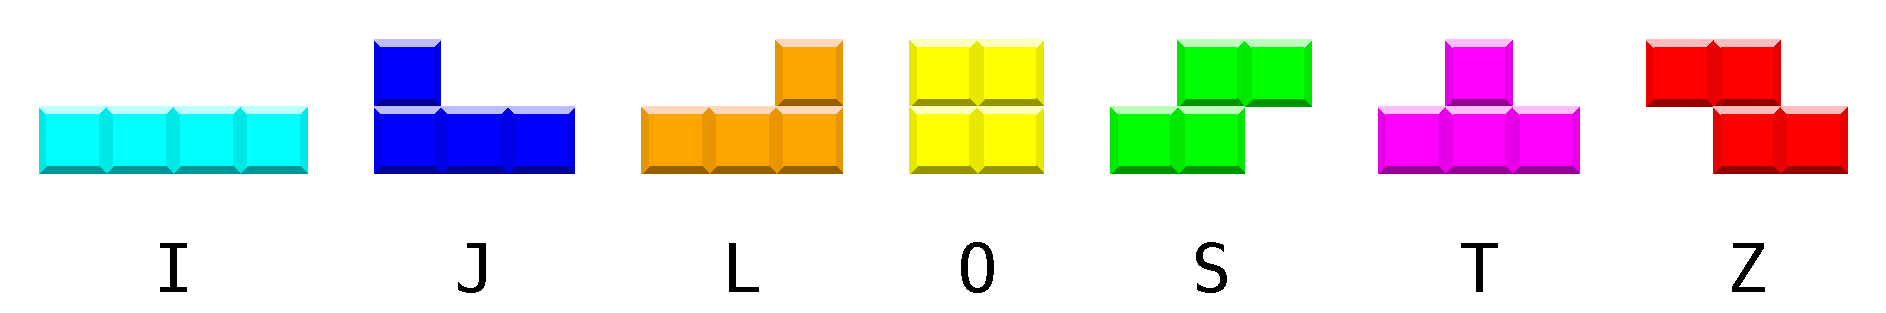
\includegraphics[width=0.8\textwidth]{all-pieces}
  \caption{The seven tetrominoes in their initial orientations.}
  \label{fig:tetris}
\end{figure}

\begin{itemize}
  \item The playing area is a grid of height $20$ and width $10$,
    initially empty.
  \item One by one, the game presents the player with a random
    sequence of tetromino shaped pieces, as seen in
    Figure~\ref{fig:tetris}. The game uses a bag randomiser for this,
    that is, the first seven pieces are all distinct, then the next
    seven pieces are distinct, and so on.
  \item The player may shift each piece sideways and rotate it by
    multiples of $90$ degrees. These adjustments take place
    \emph{above} the grid.
  \item The piece then drops down into the playing area and locks into
    place as soon as some part of it cannot drop any further because
    part of some previous piece is in the way. It is \emph{not}
    possible to shift or rotate the piece during the drop.
  \item The game ends as soon as one of the following happens:
    \begin{itemize}
      \item A horizontal row of the grid is fully occupied by
        tetromino tiles, the player wins.
      \item Some piece does not fully drop into the grid, the player
        loses.
    \end{itemize}
\end{itemize}

\section*{Interaction Protocol}

Your submission will be interacting with a special program called the
\emph{grader}. This means that the output of your submission is sent
to the grader and the output of the grader is sent to the standard
input of your submission. This interaction must follow a specific
protocol:

The grader repeatedly sends random pieces (see the note below),
denoted by one of the uppercase letters
$\{\texttt{I},\texttt{J},\texttt{L},\texttt{O},\texttt{S},\texttt{T},\texttt{Z}\}$
as in Figure~\ref{fig:tetris} above. In reply to each piece, your
submission must answer with its desired placement, in the following
format:
\begin{itemize}
  \item Two integers $r$ and $x$ ($0\le r\le 3, 1\le x\le 10$), where
    $r$ indicates how many times the piece should be rotated in
    clockwise direction, and $x$ indicates the leftmost column
    occupied by the piece (columns are indexed from left to right,
    starting at $1$).
\end{itemize}

The grader will then rotate and position the piece accordingly and
drop it in the desired location.

After sending each placement, you should \emph{flush} the standard
output to ensure that it is sent to the grader. For example, you can
use \texttt{fflush(stdout)} in C++, \texttt{System.out.flush()} in
Java, and \texttt{sys.stdout.flush()} in Python.

The game ends as soon as your submission successfully completes a row
or sends an invalid placement, whichever happens first (if both happen
at the same time, the invalid placement takes precedence).
A placement is invalid if some part of the piece would have to be
placed outside of the playing area, either to the top or to the side.

If your submission completes a row, the grader will send a single
character \texttt{W}. Upon receiving this, your submission must
terminate with exit code \texttt{0} as usual.

Your submission will be accepted if it follows the protocol above and
completes a row. If it makes an invalid placement, it will be judged
as ``Wrong Answer''.

As described above, the sequence of pieces is determined by a bag
randomiser. The seed values for this randomiser have been fixed in
advance, such that every submission is run on the same piece
sequences.

\displaysample{gameoffallingblocks/problem_statement/1}

\vspace{4mm}
In the example interaction above, one possible output of the grader is
on the left and one possible correct output of a submission is on the
right.\\
The empty lines on both sides only serve to emphasise the
chronological order. The grader will never output any empty lines.

\begin{figure}[!h]
  \centering
  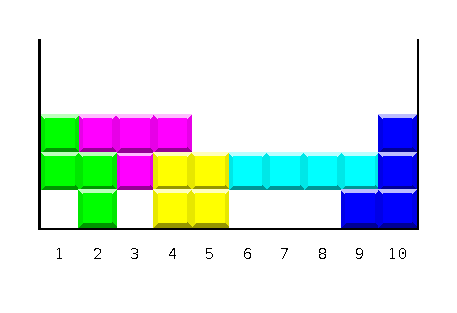
\includegraphics[width=0.5\textwidth]{sample-interaction}
  \caption{Illustration of the example interaction.}
\end{figure}
